%%%%%%%%%%%%%%%%%%%%%%%%%%%%
%\subsubsection{Physics Motivation}
%\label{sec:sp-calib-sys-pns-phys} 



The \dword{snb} signal includes low-energy  electrons, gammas and neutrons, %the final state will also include neutrons visible via 
which capture on argon. Each signal channel will have specific detector threshold effects, energy scale, and energy resolution. 
As noted in~\physchsnb, 
%Chapter~7 of Volume~\volnumberphysics~(\voltitlephysics) of this \dword{tdr},
the sensitivity to \dword{snb} physics 
depends on the uncertainties of relevant detector response parameters, and so a calibration method to constrain those uncertainties is needed.
Local detector conditions may change with time due to a variety of 
causes that include electronics noise, misalignments, fluid flow, \dword{lar} purity, electron lifetime and \efield. While these are intended to be characterized from other systems via inputs to the detector model, ``standard candles'' provide a method to assess if our detector model is incomplete or insufficient. An ideal standard candle matches one of the relevant signal processes and will provide spatial and/or temporal information. The \dlong{pns} (\dshort{pns}) system, as described below, will provide a standard candle neutron capture signal (\SI{6.1}{\MeV} multi-gamma cascade) across the entire \dword{dune} volume that is directly relevant to the supernova physics signal characterization. The \dword{pns} is also capable of providing a spatially fine-grained measurement of electron lifetime. 



Liquid argon is near transparent to neutrons with an energy near or at \SI{57}{\keV} due to an anti-resonance in the cross-section caused by the destructive interference between two high level states of the \argon40 nucleus (see Figure~\ref{fig:PNS_xsections}). The cross-section at the anti-resonance ``dip'' is about \SI{10}{\keV} wide, and at the bottom the cross section of \SI{1.6e-4}{\barn} implies an elastic scattering length of over \SI{2000}{\m}. %Of course, natural 
Natural argon has three major isotopes: \isotope{Ar}{36} (\SI{0.3336}{\%}), \isotope{Ar}{38} (\SI{0.0834}{\%}), and \isotope{Ar}{40} (\SI{99.6035}{\%}) each with a slightly different anti-resonance. The average elastic scattering length of the \SI{57}{\keV} neutrons in natural liquid argon is about \SI{30}{\m}.

\begin{dunefigure}[Cross sections enabling the \dshort{pns} concept]{fig:PNS_xsections}
{Illustration of interference anti-resonance dips in the cross section of \isotope{Fe}{56}, \isotope{Si}{28}, \isotope{S}{32}, and \isotope{Ar}{40}. Elastic scattering cross-section data is obtained from ENDF VIII.0~\cite{Brown:2018jhj}.}
%Brown:2018jhj}.} - it was BROWN20181 (AH 7/29/20; fixed for JINST)
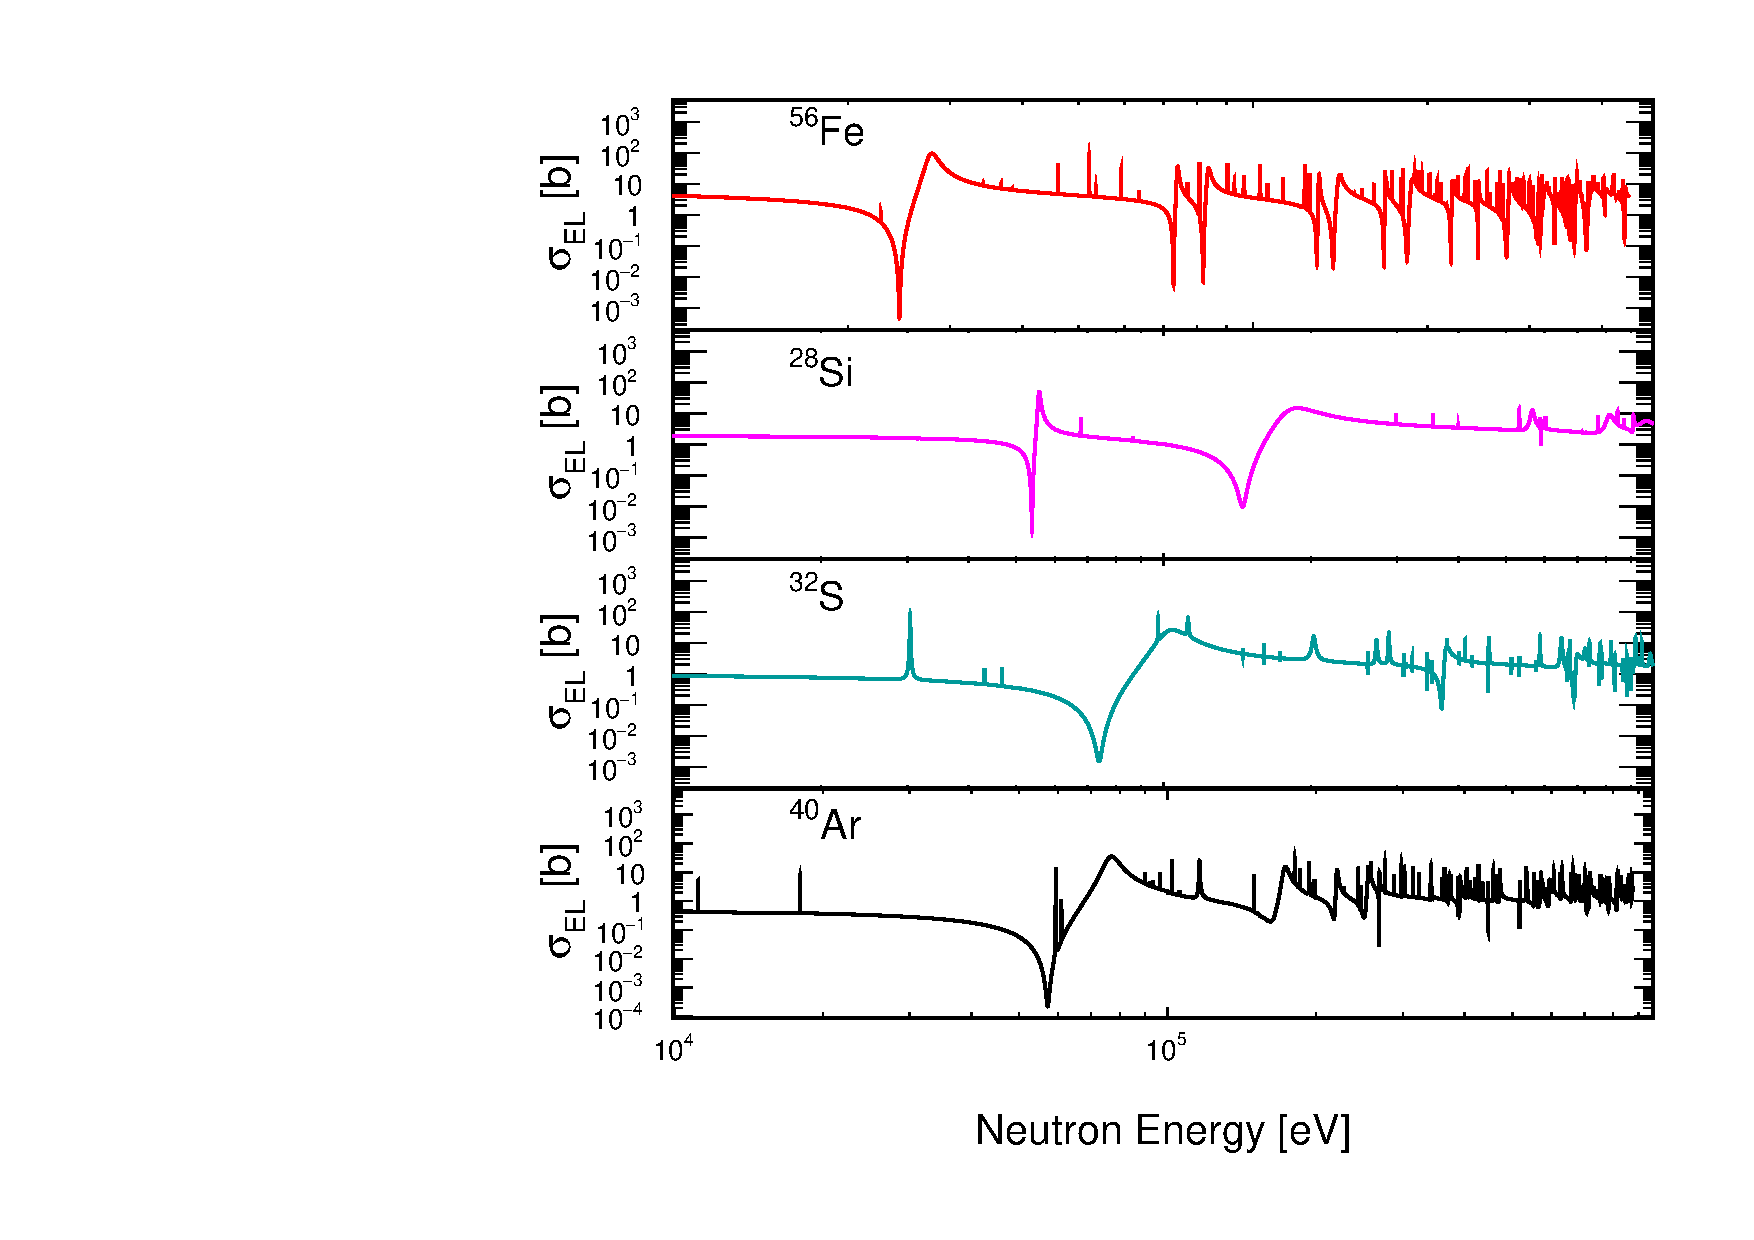
\includegraphics[width=10cm]{graphics/PNS_xsection.pdf}
\end{dunefigure}
%\fixme{need ref: endf viii}

The neutrons at the anti-resonance energy could be injected into liquid argon in the \dword{tpc}, provided no materials (e.g., hydrocarbons) block the path. Those that do scatter lose energy, leave the anti-resonance, quickly slow down and are captured. Each capture releases exactly the binding energy difference between \isotope{Ar}{40} and \isotope{Ar}{41}, about \SI{6.1}{\MeV} in the form of $\gamma$ rays.  As will be described below, by using a $DD$ Generator (where $DD$ stands for ``deuterium-deuterium''), a triggered pulse of neutrons can be generated outside the \dword{tpc}, then injected via a dedicated opening in the insulation into the liquid argon, where it spreads through the \SI{58}{\m} volume of the detector to produce \SI{6.1}{\MeV} energy depositions.

One important property of the neutron capture reaction \isotope{Ar}{40}(n,$\gamma$)\isotope{Ar}{41} is that the deexcitation of \isotope{Ar}{41} nucleus produces a cascade of prompt $\gamma$s. Because of the detector threshold effect, the multiplicity and the
total energy of the $\gamma$s within the cascades could be effectively decreased to below the expected values of the neutron capture process. As a consequence, the neutron capture identification and the assessment of neutron tagging efficiency in liquid argon strongly depends on a precise model of the full $\gamma$ energy spectrum from thermal neutron capture reaction. The neutron capture cross-section and the $\gamma$ spectrum have been measured and characterized by the Argon Capture Experiment at DANCE (ACED), where DANCE is the Detector for Advanced Neutron Capture Experiments. Recently, the ACED collaboration performed a neutron capture experiment using DANCE at the Los Alamos Neutron Science Center (LANSCE). The result of neutron capture cross-section was published~\cite{Fischer:2019qfr} and will be used to prepare a database for the neutron capture studies. The data analysis of the energy spectrum of correlated $\gamma$ cascades from neutron captures is underway and will be published soon. 
The $\gamma$ energy spectrum and the branching ratios in the ENDF library will be updated with the ACED result. 

Figure~\ref{fig:PNS_gamma_ACED_v2} shows an example of the energy spectra of individual $\gamma$ clusters measured by ACED~\cite{Fischer:2019qfr}. The most common $\gamma$ cascade emitted from \isotope{Ar}{41} decay has \SI{167}{keV}, \SI{1.2}{MeV} and \SI{4.7}{MeV} $\gamma$s. The peak energy of these $\gamma$s can be clearly seen in the background subtracted data in Ref.~\cite{Fischer:2019qfr}. In liquid argon detectors, the $\gamma$s are detected through calorimetric measurement. Assuming the $\gamma$ cascade from a neutron capture is fully contained in the active volume, it is possible to detect the individual $\gamma$s from the neutron capture. The correlation of the measured $\gamma$ is a strong indication of neutron capture events. Low energy $\gamma$ reconstruction algorithms are being investigated to identify the neutron capture events that could be used for detector response calibration. 

%aced replaced with Fischer:2019qfr
\begin{dunefigure}[Neutron capture gamma spectrum measured by ACED]{fig:PNS_gamma_ACED_v2}
{Energy spectra of individual $\gamma$ clusters measured by ACED. Only events detected in the \SIrange{0.02}{0.04}{eV} neutron energy window are selected.}
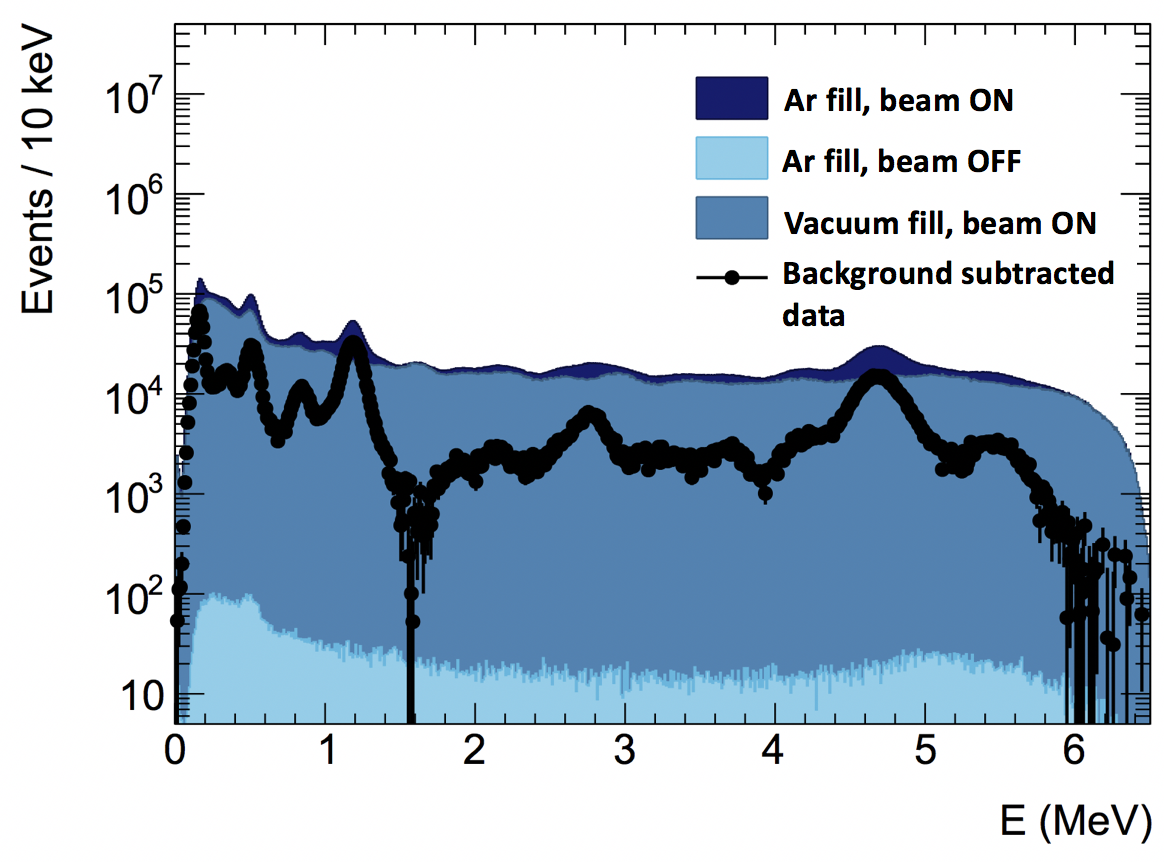
\includegraphics[width=10cm]{graphics/PNS_gamma_ACED_v2.png}
%graphics/PNS_gamma_spectrum_ACED.png}
\end{dunefigure}

%{\it Mention Test at LANSCE and its role?}

%%%%%%%%%%%%%%%%%%%%%%%%%%%%
\subsubsection{Design}
\label{sec:sp-calib-sys-pns-des}

The basic design concept of sources like the \dlong{pns} are based on successful boron neutron capture therapy~\cite{bib:Koivunoro2004}. The design of the \dword{pns} system used for energy calibration is shown in Figure~\ref{fig:PNS_Moderator}. The system will consist of four main components: a $DD$ generator, an energy moderator reducing the energy of the $DD$ neutrons down to the desired level, shielding materials, and a neutron monitor to confirm neutron flux and safe operation. 

\begin{dunefigure}[Conceptual design of the \dshort{pns}]{fig:PNS_Moderator}
{Conceptual design of the \dlong{pns}. The whole device is placed outside the \dword{tpc} volume on top of the cryostat.}
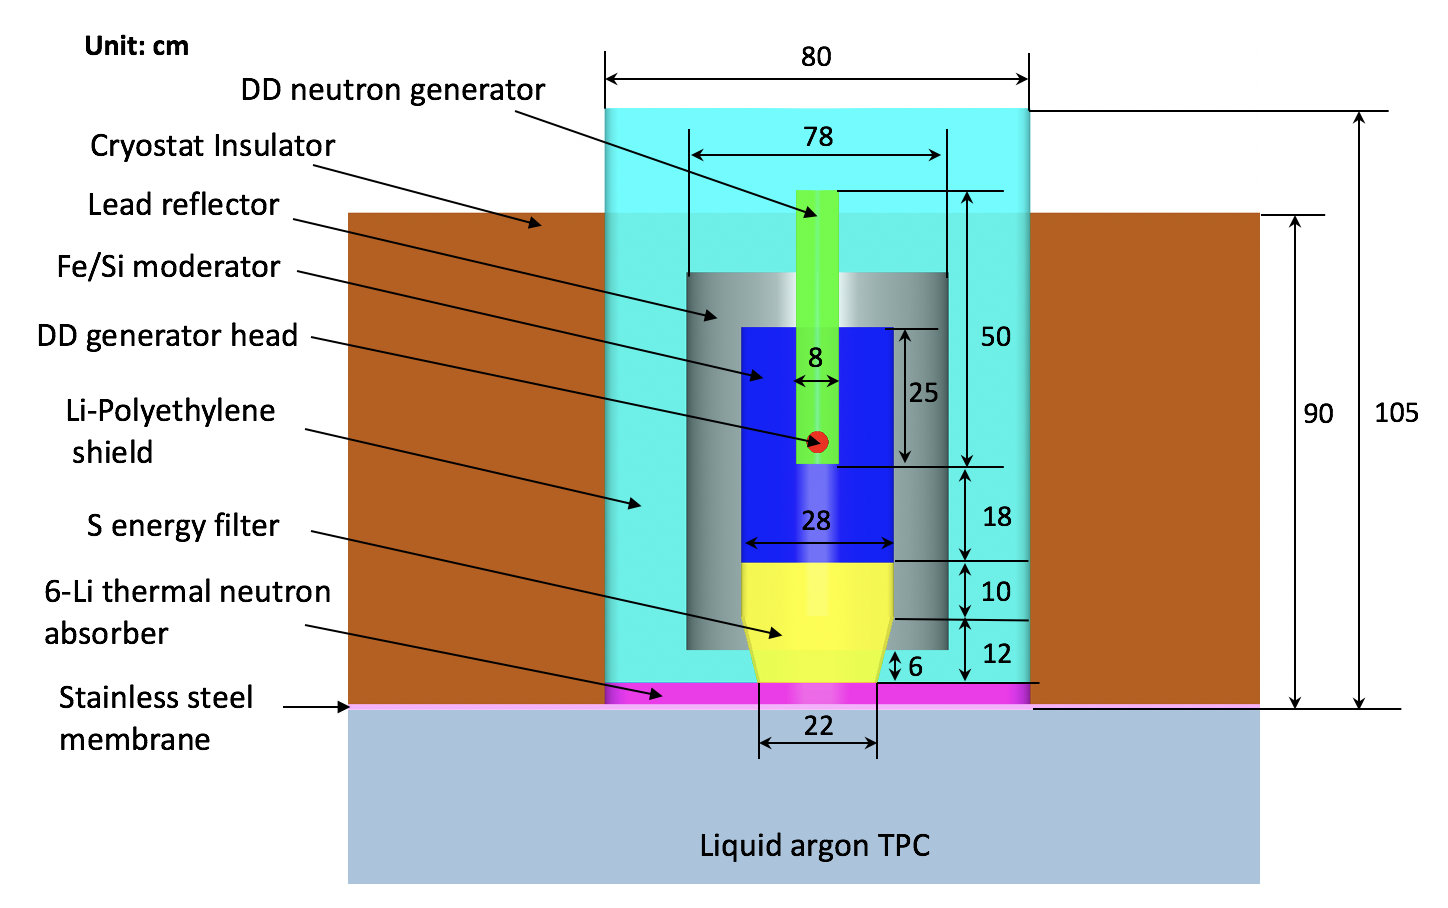
\includegraphics[width=12cm]{PNS_Moderator.png}
\end{dunefigure}

{\bf DD generator source:} $DD$ generators are commercial devices that can be readily obtained from several vendors at a cost of about \$\num{125}k each, which includes all control electronics. The pulse width is adjustable and can be delivered from about \SIrange{10}{1000}{\micro\s} (which affects the total neutron output). 

{\bf Moderator:}  A feasible moderator has been designed using a layered moderator~(Fe or Si)-filter~(S)-absorber~(Li) %layered 
configuration. The \SI{2.5}{\MeV} neutrons from the $DD$ generator are slowed to less than \SI{1}{\MeV} by the energy moderator. Natural iron and silicon are found to be efficient moderators for this purpose. Then an energy filter made of sulfur powder is used to further select the neutrons with the desired anti-resonance energy.
The neutron anti-resonance energy in \isotope{S}{32} is \SI{73}{\keV}, right above the \SI{57}{\keV} anti-resonance energy in \argon40. The neutrons at this energy lose about \SI{3.0}{\keV} per elastic scattering length. After a few elastic scattering interactions, most of the \SI{73}{\keV} neutrons selected by the sulfur filter will fall into the \SI{57}{\keV} anti-resonance energy region in \dword{lar}. These materials require no cooling or special handling. Finally, a thermal absorbing volume of lithium is placed at the entry to the argon pool in order to capture any neutrons that may have fallen below the \SI{57}{\keV} threshold. A reflecting volume is added around the $DD$ generator and the neutron moderator to increase downward neutron flux. Figure~\ref{fig:PNS_Energy_Moderator} shows the energy spectrum of the neutrons moderated and injected into the \dword{tpc}.


\begin{dunefigure}[Energy of moderated neutrons produced by the \dshort{pns}]{fig:PNS_Energy_Moderator}
{Energy of moderated neutrons produced by the \dlong{pns}. %Simulation is based on Design A shown in Figure~\ref{fig:PNS_Two_Designs}. 
The total number of initial $DD$ generator neutrons is \num{1e6}.}
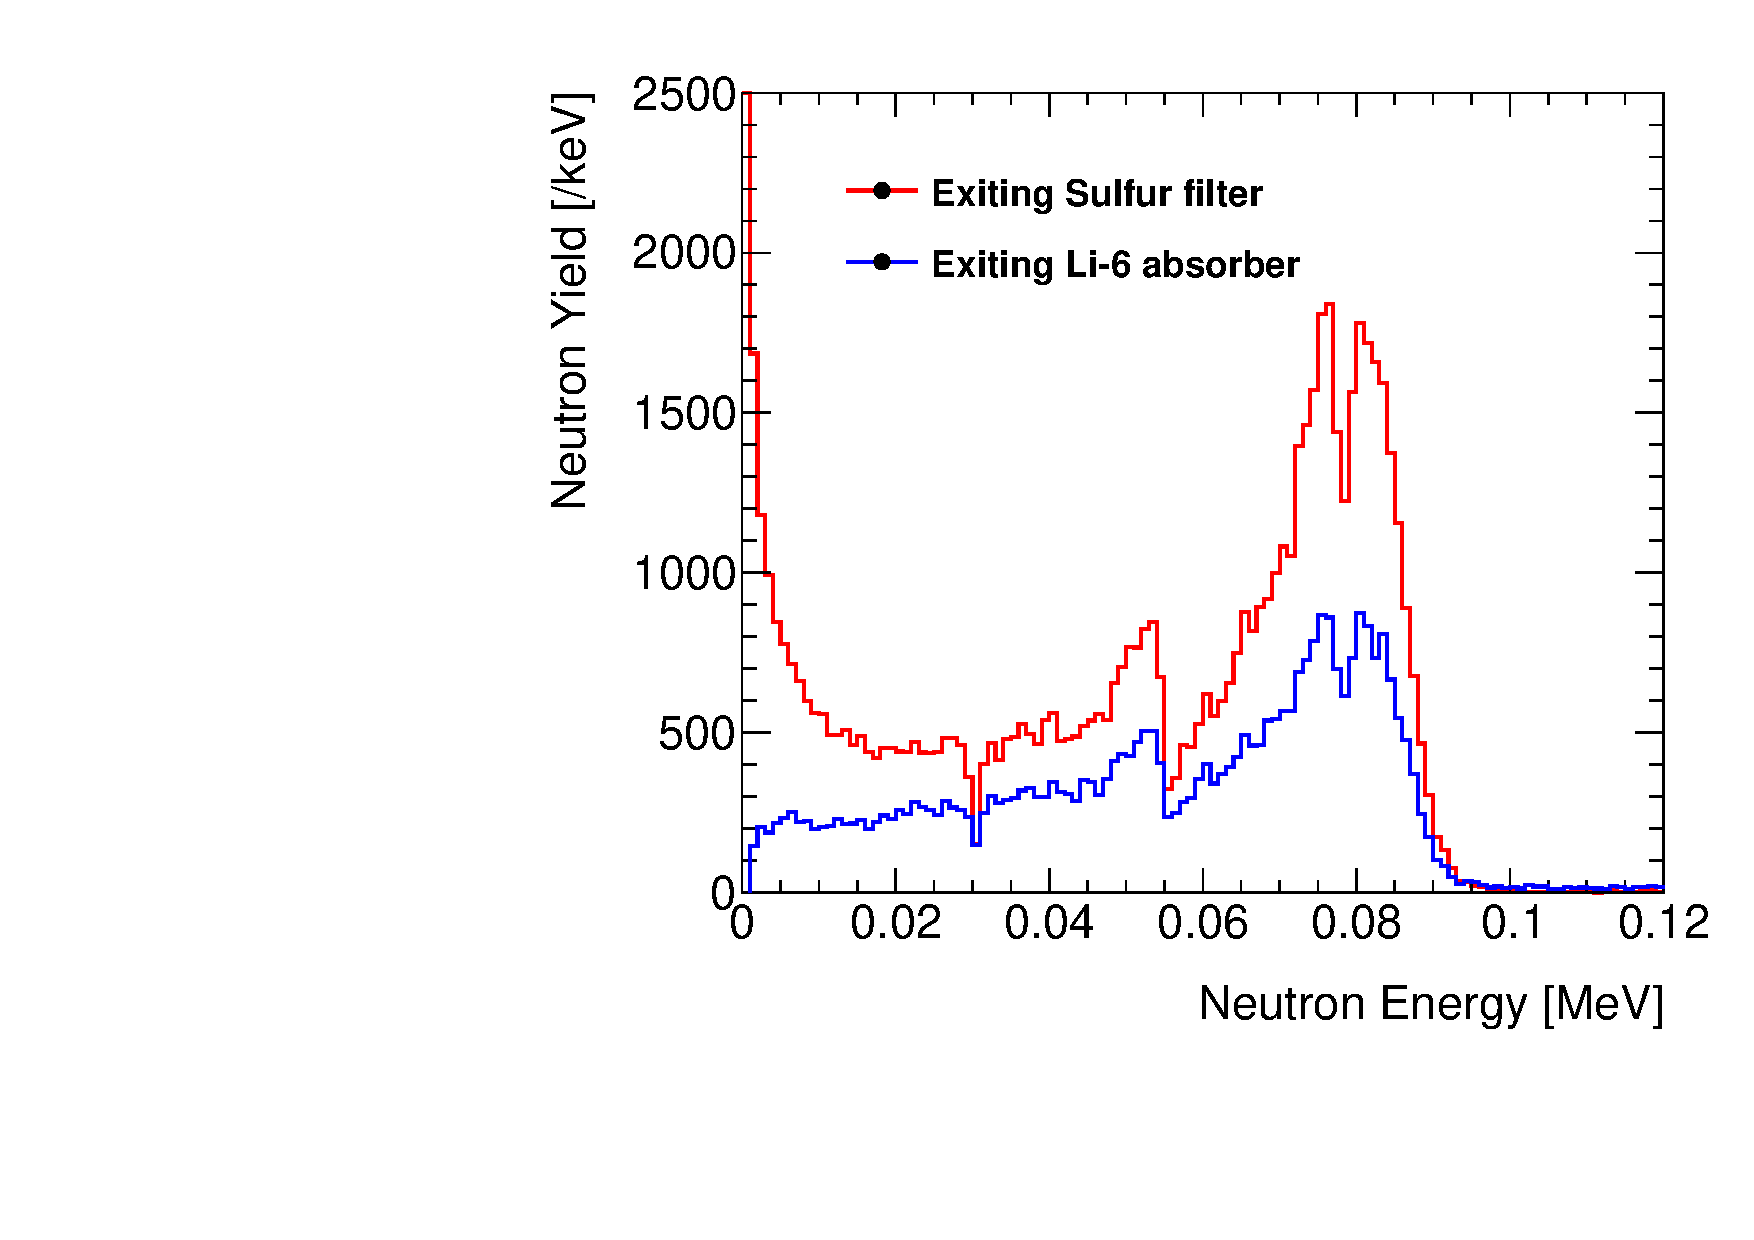
\includegraphics[width=9cm]{PNS_Energy_Moderator.pdf}
\end{dunefigure}

{\bf Shielding:} The source will be encased in a shielding volume. The goal of the shield is to block both scattered neutrons and gammas that are produced in the source. Lithium-polyethylene (\SI{7.5}{\%}) is chosen to be the material for the neutron shield because it is rich in hydrogen and lithium atoms which yield a high neutron absorption cross section. Lithium-polyethylene is also light weight, commercially available, and relatively inexpensive. The energy spectrum entering the shield has multiple peaks between \SI{0.5}{\MeV} and \SI{1.5}{\MeV}, and one major spike at \SI{2.2}{\MeV}. The shield can effectively block the lower energy peaks but can only degrade the intensity of the \SI{2.2}{\MeV} because \SI{2.2}{\MeV} gammas are a characteristic signature for neutron captures on hydrogen. A safe thickness of the lithium-polyethylene shield must be found, one that can degrade the dose of \SI{2.2}{\MeV} gammas to safe levels. The dose of radiation from \SI{2.2}{\MeV} gammas was calculated assuming a person standing \SI{1}{\m} away. Simulation indicates that a shield with \SI{12}{\cm} thick lithium-polyethylene satisfies basic safety requirements\footnote{These calculations will be redone assuming a \SI{30}{\cm} personnel safety distance and shielding thickness reestimated to meet \dword{dune} safety requirements.}. 

 
{\bf Neutron Monitor:} The system will need a monitoring system to confirm that the source is operating as expected.  A neutron monitoring detector consisting of an Eljen EJ-420 coupled to an ADIT L51B16S \num{2}-inch \dword{pmt} will be placed just outside of the moderating material surrounding the $DD$ generator and will be read out with a CAEN waveform digitizer with neutron/$\gamma$ pulse-shape discriminating firmware. The monitoring detector will provide relative flux information to the calibration users and will ensure that the intensity of the source is constant, thereby allowing a comparison of data taking at different times.  A small collimator will be placed in front of the neutron detector, and inside the shielding material of the $DD$ source. The collimator dimensions and material specifications (likely a combination of iron, lead, and polyethylene) will be optimized from Monte Carlo simulations.

Based on the general concept described above, Figure~\ref{fig:PNS_Moderator_largeformat} shows a conceptual layout of the neutron injection system. It is referred to as the ``large format moderator'' design. The neutron source is about \SI{0.8}{\m} wide and \SI{1}{\m} high. It would sit above the cryostat insulator. Beneath the neutron source, a cylindrical insulator volume with a diameter of more than \SI{50}{\cm} has to be removed to allow the neutrons enter the cryostat. Such an interface is provided by the human access ports near the endwalls of the detector.
%; a picture of this is shown for \dword{protodune} in Figure~\ref{fig:manhole2}. 
The top flange of the human access port is sealed, and the neutron source sits on top, providing heat insulation. The neutron source weighs about \SI{1.6}{\tonne} and will be supported by the I-beams. 
This design allows a permanent deployment of the neutron source. GEANT4 simulation has shown that \SI{0.13}{\%} of the neutrons generated by the $DD$ generator are expected to be captured inside the \dword{tpc}. It is also possible to place the neutron source inside the human access ports which would allow a factor of \num{6} increase of the neutron flux but will require a modification of the interface flange. This is currently being investigated.

%\begin{dunefigure}[\dword{pns_baseline}
%]{fig:PNS_baseline}
\begin{dunefigure}[\dshort{pns} baseline design]{fig:PNS_Moderator_largeformat}
{Large format neutron source deployed above/inside the human access holes.}
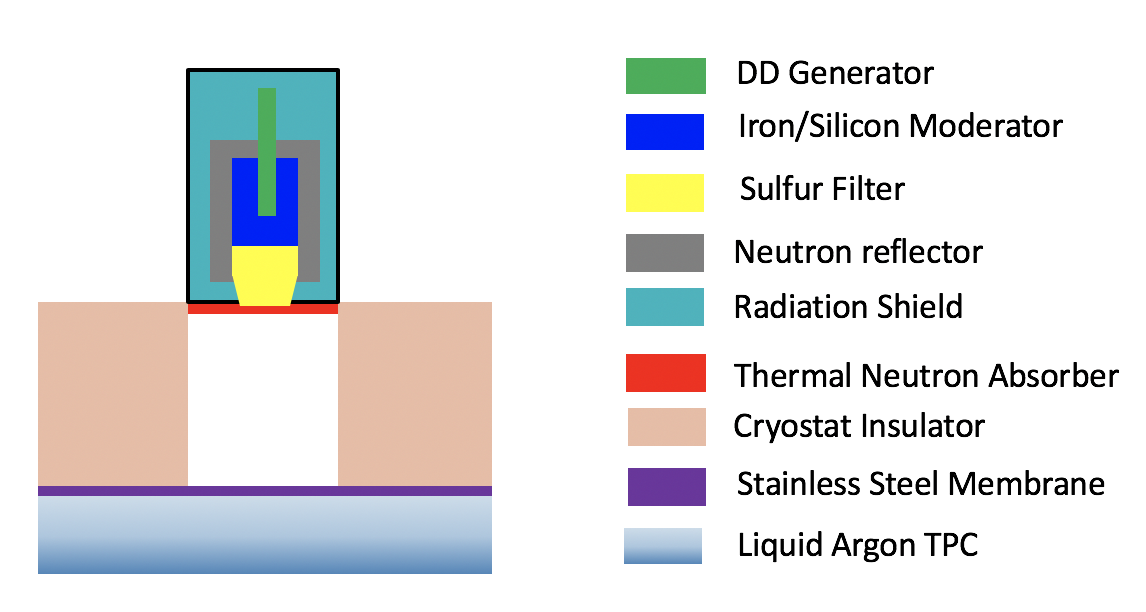
\includegraphics[width=12cm]{PNS_Moderator_largeformat.png}
\end{dunefigure}



Simulation studies were done placing the \dword{pns} system on top of a cryostat with the same size as the \dword{dune} \SI{10}{\kton} \dword{tpc}. Initial simulation results indicate that one \dword{pns} could cover 1/3 of the \dword{tpc} volume, so three identical neutron sources on top of the cryostat would illuminate the whole \dword{tpc} volume of the \dword{dune} \dword{fd}. However, this would require opening three additional neutron injection ports which are not included in the current cryostat design\footnote{Ideally, opening three identical neutron injection ports for each \SI{10}{\kton} TPC would make full use of the neutron source. While this is not possible for the first \dword{fd} module as the cryostat design is frozen, it informs the importance of these ports for subsequent \dword{fd} modules.}. The baseline configuration of the \dword{pns} system consists of two large format neutron sources permanently located at the corner human access ports at the opposite ends on top of the cryostat. 

Figure~\ref{fig:PNS_ncapDistribution_two_sources} shows the position distribution of the neutron captures under baseline configuration. The distribution shows that the baseline deployment can cover a large fraction of the \dword{tpc} volume, but, as evident from the figure, not many neutrons reach the central region of the \dword{tpc}. Neutrons with long scattering lengths can reach the center of the \dword{tpc} but, much longer operation time maybe needed to achieve the required statistics. Assuming a minimum number of \num{100} neutron captures per \si{\cubic\m} in order to carry out a localized energy calibration, and the typical $DD$ generator pulse intensity of \num{e5} neutrons/pulse, the number of pulses needed to calibrate the high rate regions is of the order of \num{1000}, and at least \num{10} times that for the low rate regions. But given the \SI{0.5}{\hertz} \dword{daq} limitation, this would mean calibration runs will increase from 40 minutes to about \num{7} hours to cover the low rate regions. More details on this are given in Section~\ref{sec:sp-calib-daqreq}.
If the neutron capture events at the center of the \dword{tpc} are not sufficient, the detector response calibration would depend on simulations and extrapolation using results from the regions with high neutron coverage. To increase the low coverage at the center of the \dword{tpc}, an alternative deployment strategy is proposed using a small format neutron source design described in Section~\ref{sec:sp-calib-pns-alter}. 

\begin{dunefigure}[Pulsed neutron system neutron capture positions inside a \dshort{dune}-sized \dshort{tpc}]{fig:PNS_ncapDistribution_two_sources}
{Neutron capture positions inside a \dword{dune}-sized \dword{tpc}, assuming baseline configuration with two large format neutron sources located at the corner human access ports at the opposite corners on top of the cryostat. $L$=\SI{60}{\m} (along $Z$ axis, horizontally parallel to the beam direction), $W$=\SI{14.5}{\m} (along $X$ axis, horizontally perpendicular to the beam direction), $H$=\SI{10}{\m} (along $Y$ axis, vertically perpendicular to the beam direction). \num{1.8e7} $DD$ generator neutrons with \SI{2.5}{\MeV} energy were simulated in each moderator and propagated inside the \dword{tpc}. Top (left) and side (right) views of neutron capture positions are shown.}
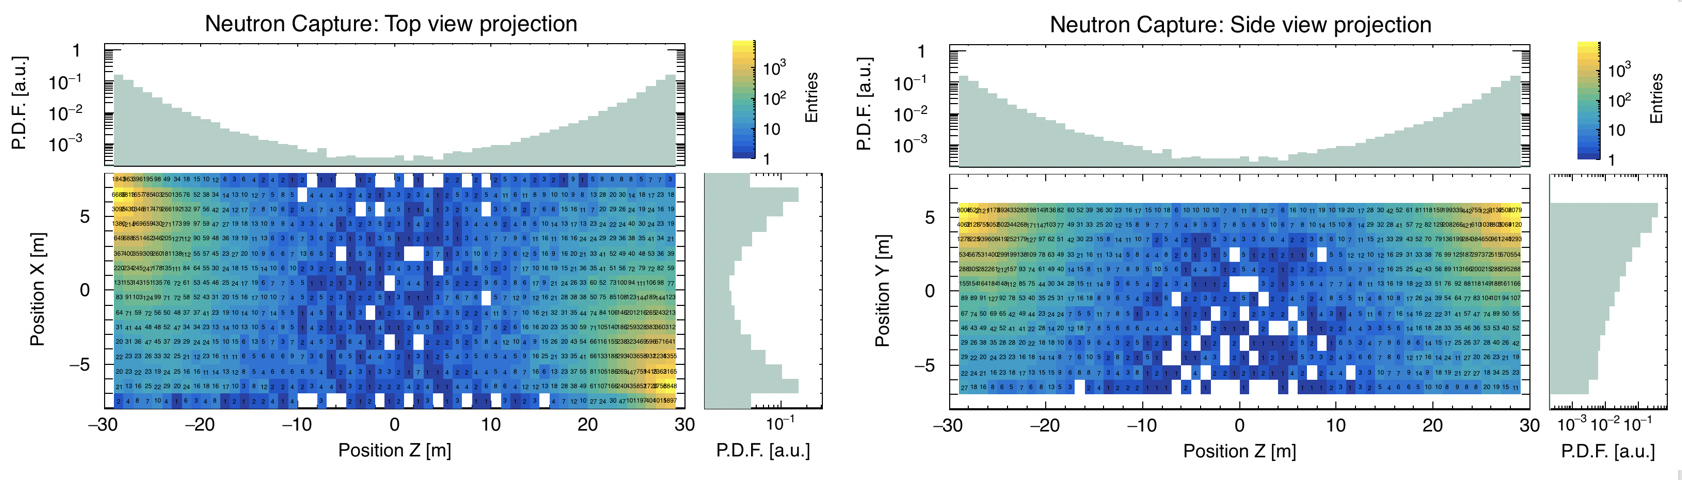
\includegraphics[width=18cm]{PNS_ncapDistribution_two_sources.png}
%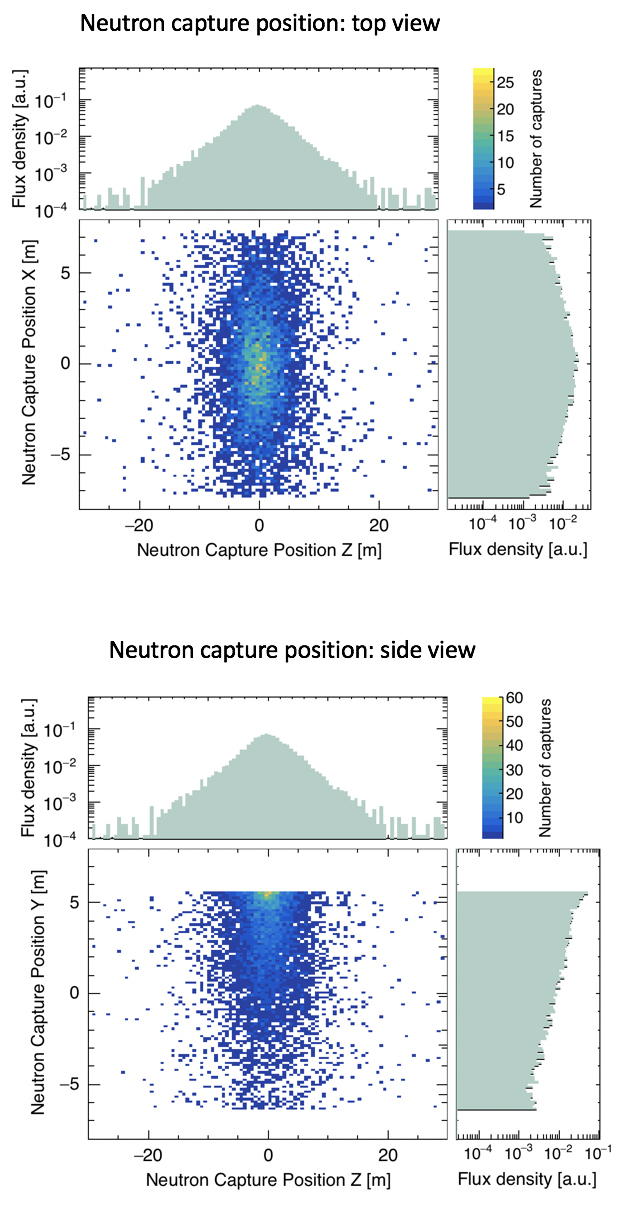
\includegraphics[width=10cm]{PNS_NcapPosition_v2.png}
\end{dunefigure}

The system is expected to have a long lifetime of operation, as the \dword{pns} system sits on top of the cryostat, with no opening to the \dword{lar}, so it is possible to replace the system in case of failure with only crane support.

%%%%%%%%%%%%%%%%%%%%%%%%%%%%

%%%%%%%%%%%%%%%%%%%%%%%%%%%%%%%%%%

%%%%%%%%%%%%%%%%%%%%%%%%%%%%
\subsubsection{Measurement Program}
\label{sec:sp-calib-sys-pns-meas}

The \SI{6.1}{\MeV} $\gamma$ cascade will provide a uniform signal for neutron capture, part of the supernova signal. The source may also be used to determine the relative efficiency across the detector for neutron capture, and provide measurements of energy resolution and energy scale spatially and temporally. Simulation studies are currently underway.
%and for the second draft, we plan to include a first round of simulation results.

%\todo{Simulation studies are underway but changing rapidly. for v2 we will include a first round of studies.}

The first goal of the simulation is to provide the expected distribution of signals, with a normalization given by the pulse width of \dword{pns} operation, and neutrons energy and angular correlated distribution, depending on the source filter and shield design.
%which can also be used to optimize the calibration strategy.
%. It will be used to optimize the calibration strategy too. 
It is envisaged that the calibration can be done in two modes. First, a short \dword{pns} pulse can provide isolated neutron captures closer to the entrance path; and then a longer 
%\dword{pns} 
pulse, for which the same region is saturated, but 
%isolated neutron 
captures 
%can be obtained 
happen in the full volume.

By using an external trigger coupled to the \dword{pns} operation and running the usual trigger algorithms in parallel, the calibration will provide the efficiency of the trigger and \dword{daq} systems as a function of total fluxes. Changing the pulse width can result in 
%resulting on 
higher or lower detector activity. The source will be used for \dword{snb} calibration to test
%, in the sense of testing 
the capabilities of triggering for low energy signals, but also 
%of identifying 
to identify them in different pile-up conditions.
The transmission of the global timing from the external \dword{pns} trigger to the \dword{daq} provides a strong constraint on the initial timing for the \dword{tpc}
%Time Projection Chamber 
as the neutron capture times are of the order of \SI{0.15}{\milli\s}, much lower than typical drift time 
%scale 
for the TPC. The \dword{pds}, with resolution of \SI{100}{\nano\s}, can discriminate between different neutron captures. The calibration will measure the efficiency of the \dword{pds} response for low energy events, depending on the distance due to Rayleigh scattering in \lar. We will then study the usage of the \dword{pds} time information for improving the position reconstruction of \dword{tpc} signals. In the absence of the \dword{pds} system, the global timing from the \dword{pns} translates to an uncertainty of around \SI{10}{\cm}.

Individual event positions can be translated into response maps of both the photon detectors and the \dword{lartpc} to standard candles of \SI{6.1}{\MeV} electromagnetic depositions. When the cascades can be more precisely reconstructed, individual $\gamma$s within the cascades can be identified, and this provides a lower energy ``standard candle'' close to the solar electron-neutrino threshold. Comparing the collected charge for equal energy signals at different distances from the \dword{tpc} gives a measurement of the electron lifetime, a key detector response parameter. High \dword{pns} flux runs can generate momentary local space charge effects, in the 
%top parts 
upper regions of the detector, that will need to be characterized; low flux runs should be taken before to ensure %usual 
expected space charge distributions.
The global simulation will be tested in the (smaller scale) \dword{protodune} detectors. The neutron mean free path will be larger than the \dword{protodune} size, and so 
%there will be more 
external events and interactions with materials of the \dword{pds}, \dword{apa}, and \dword{cpa} systems will be more prominent. These effects must be simulated.

%Notice 
Note that captures of external background neutrons, entering the active volume is a main background for low energy physics; a comparison of simulations of \dword{pns} events and external neutron backgrounds will be interesting, as will a comparison of simulated supernova and solar neutrino signals. For the high energy beam events, the number and energy distributions of neutrons depend on the type of neutrino interaction and are significantly different for neutrinos and anti-neutrinos. Measuring the number and distance of neutron captures around the main hadronic cascades can thus help in identifying which extra proton scattering signals to associate to the hadronic cascades. This can also help make a statistical correction to the energy reconstruction of the neutrino and anti-neutrino events.




